The OpenQuake-engine offers the possibility of calculating seismic hazard and loss (or risk) maps. To do so, it utilizes the seismic hazard or loss exceedances curves, to estimate the corresponding hazard or loss for the pre-defined return period (or probability of exceedance within a given interval of time).

\subsection{Plotting hazard maps}
\label{subsec:plot-hazard_maps}
A seismic hazard map provides the expected ground motion (e.g. peak ground acceleration or spectral acceleration) at each location, for a certain return period (or probability of exceedance within a given interval of time). To plot this type of maps, it is necessary to specify the location of the output file using the parameter \verb=hazard_map_file=. An example hazard map is displayed in Figure \ref{fig:hazard_curve}.

\begin{figure}[htb]
  \centering
      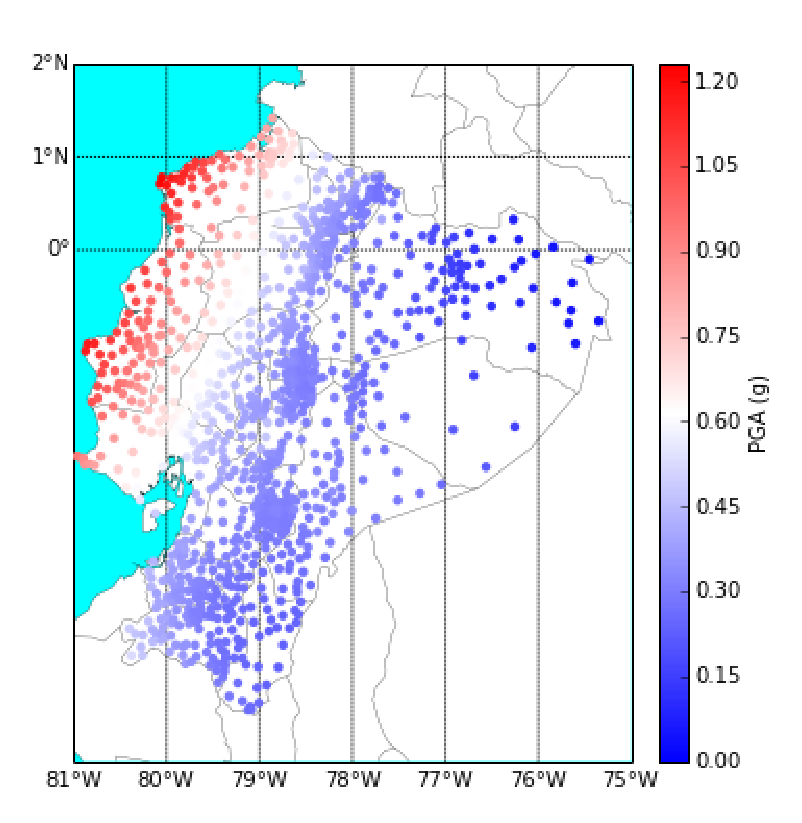
\includegraphics[width=7cm]{figures/hazard_Ecuador.eps}
  \caption{Seismic hazard map for a probability of exceedance of 10\% in 50 years.}
  \label{fig:hazard_map}
\end{figure}

\subsection{Plotting loss maps}
\label{subsec:plot-loss_maps}
A loss map provides the estimated losses for a collection of assets, for a certain return period (or probability of exceedance within a given interval of time). It is important to understand that these maps are not providing the distribution of losses for a seismic event for the chosen return period, nor the losses whose sum would correspond to the aggreagted loss for the same return period. This type of maps is simply providing the expected loss for a specified level of frequency for each asset. 
To use this feature, it is necessary to define the parth ot the output file using the parameter \verb=loss_map_file=, as well as the exposure model used to perform the risk calculations through the parameter \verb=exposure_model=. Then, similarly to what was explained in section \ref{subsec:plot-collapse_maps} for collapse maps, it is possible to follow three approaches to generate the loss maps:\\ 

\begin{enumerate}
\item Aggregated loss map only.
\item Loss maps per taxonomy only.
\item Both aggregated and taxonomy-based.\\
\end{enumerate}

Then, there are a number of options that can be used to modify the style of the maps. These include the size of the marker of the map (\verb=marker_size=), the geographical limits of the map (\verb=bounding_box=), and the employment of a logarithmic spacing for the color scheme (\verb=log_scale=). An example loss map for a single vulnerability class is presented in Figure \ref{fig:loss_map}.

\begin{figure}[htb]
  \centering
      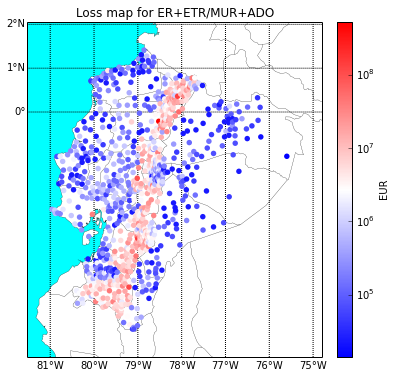
\includegraphics[width=7cm]{figures/loss_map.png}
  \caption{Loss (economic) map for a probability of exceedance of 10\% in 50 years.}
  \label{fig:loss_map}
\end{figure}

As mentioned on the introductory section, it is also possible to convert any of the maps into a format (csv) easily readable by GIS software. To do so, it is necessary to set the parameter \verb=export_map_to_csv= to \verb=True=. As an example, a map containing the average annual losses for Ecuador has been converted to the \verb=csv= format, and introduced into the QGIS software to produce the map presented in Figure \ref{fig:all_loss_map}.

\begin{figure}[htb]
  \centering
      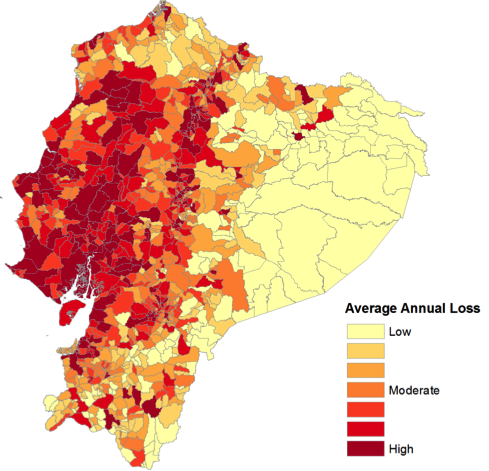
\includegraphics[width=6cm]{figures/loss_map_AAL.png}
  \caption{Average annual (economic) losses for Ecuador.}
  \label{fig:all_loss_map}
\end{figure}
